\documentclass[10pt,twocolumn,letterpaper]{article}

\usepackage{cvpr}
\usepackage{times}
\usepackage{epsfig}
\usepackage{graphicx}
\usepackage{amsmath}
\usepackage{amssymb}

% Include other packages here, before hyperref.
\usepackage{float}
\usepackage{multirow}
\usepackage[export]{adjustbox} % https://tex.stackexchange.com/questions/57418/crop-an-inserted-image

% If you comment hyperref and then uncomment it, you should delete
% egpaper.aux before re-running latex.  (Or just hit 'q' on the first latex
% run, let it finish, and you should be clear).
\usepackage[pagebackref=true,breaklinks=true,letterpaper=true,colorlinks,bookmarks=false]{hyperref}

%\cvprfinalcopy % *** Uncomment this line for the final submission

\def\cvprPaperID{1337} % *** Enter the CVPR Paper ID here
\def\httilde{\mbox{\tt\raisebox{-.5ex}{\symbol{126}}}}

% Pages are numbered in submission mode, and unnumbered in camera-ready
\ifcvprfinal\pagestyle{numbered}\fi

% My stuff
\hyphenation{vSLAM}

\begin{document}

%%%%%%%%% TITLE
\title{Convolutional Neural Networks for Loop-Closure Detection in vSLAM Systems}

\author{Zachariah Carmichael\\
Rochester Institute of Technology\\
Rochester, NY, USA\\
{\tt\small zjc2920@rit.edu}
% For a paper whose authors are all at the same institution,
% omit the following lines up until the closing ``}''.
% Additional authors and addresses can be added with ``\and'',
% just like the second author.
% To save space, use either the email address or home page, not both
}

\maketitle
%\thispagestyle{empty}

%%%%%%%%% ABSTRACT
\begin{abstract}
  Loop-closure detection is one of the most critical problems that visual simultaneous localization and mapping (vSLAM) systems need to mitigate. In conventional systems, hand-crafted features are used 
with a similarity metric to determine whether a loop-closure has occurred. Convolutional neural networks (CNNs) have been shown to extract more robust features, and various convolutional neural network 
architectures have been used successfully in place of hand-crafted features. In this work, extracted features from the \textup{OverFeat} CNN architecture were utilized to predict loop closures in several 
\textup{Oxford Robotics} vSLAM datasets. The results exhibit that obtained similarity matrices are indicative of similar pairwise images and could be viable for use in a vSLAM system.
\end{abstract}

%%%%%%%%% BODY TEXT
\section{Introduction}
vSLAM systems comprise two primary components: visual odometry and global map optimization \cite{taketomi_visual_2017}. Loop-closure detection algorithms are used in order to determine when to perform 
the latter component. The objective of such methods is to detect a loop-closure, \textit{i.e.} a spatial position that has already been visited by an agent. Using this location as a reference, the stored 
data structure, such as a graph, can be aligned with previously incorporated frames to more reliably and consistently determine agent location, as well as lessen map complexity. Many variants of SLAM 
systems have been introduced with a range of sensors and algorithms. LIDAR-based systems dominated the literature for years and have been shown to be effective 
\cite{levinson_robust_2010,levinson_map-based_2007}, but were inherently expensive. With motivation to reduce costs and implementation complexity, vSLAM emerged and focused on the practical use of 
monocular, stereo, and RGB-D cameras.

\begin{figure}
\centering
% \includegraphics[width=0.9\linewidth]{new_college_comparison.eps}
\adjincludegraphics[trim={2cm 2.2cm 1.5cm 2.4cm},clip,width=0.86\linewidth]{simplot_w_gt_college_inception_v1.png}
\caption{Loop-closure similarity matrix compared to ground truth for \textit{New College} dataset.}
\label{fig:new_college_sim}
\end{figure}

% In vSLAM methods, there are three primarily derived methods: feature-based, direct, and RGB-D \cite{taketomi_visual_2017}. Feature-based methods use explicitly extracted features from visual input data 
as input to the vSLAM system. ORB-SLAM \cite{mur-artal_orb-slam:_2015} is described as one of the most complete monocular vSLAM systems \cite{taketomi_visual_2017} which uses these hand-crafted features. 
In direct methods, the entire input space is used without explicit feature extraction. LSD-SLAM \cite{engel_lsd-slam:_2014} directly operates on images by recreating a synthetic scene with estimated 
depth information based on high-intensity gradients. This work focuses on classifying loop-closures for RGB data only and approaches the problem differently than any of the aforementioned methods.

Rather than using traditionally utilized hand-crafted features, this work extracts feature vectors from a pre-trained CNN. Feature vectors are pre-processed before computing pairwise image similarity 
that is thresholded to indicate whether a loop-closure has occurred. The rest of this paper is organized as follows. After the introduction, Section \ref{sec:background} provides background information. 
Section \ref{sec:method} presents the proposed model. Section \ref{sec:results} introduces the dataset, mode of evaluation, and results obtained on the \textit{New College} and \textit{City Centre} 
datasets. Section \ref{sec:conclusion} contains concluding remarks.

%-------------------------------------------------------------------------
\section{Background}
\label{sec:background}

\begin{figure*}
\centering
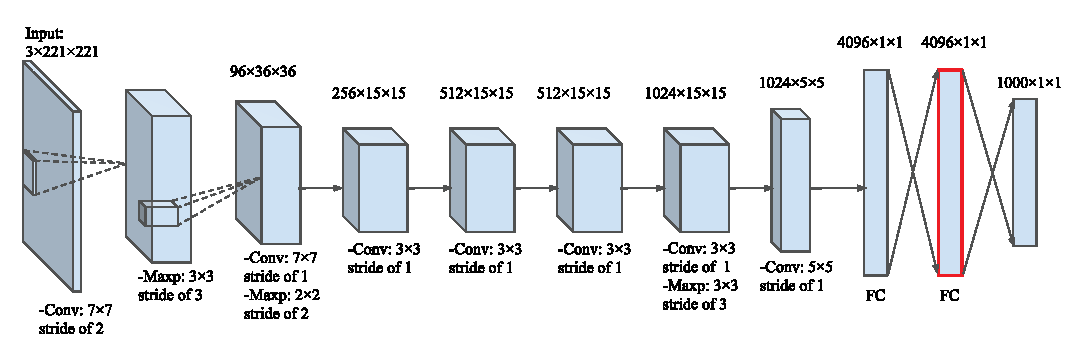
\includegraphics[width=0.72\linewidth]{DEEPSLAM.eps}
\caption{The \textit{OverFeat accurate} CNN architecture \cite{zhang_loop_2017}. Feature vectors are extracted from the first fully-connected (FC) layer.}
\label{fig:DEEPSLAM}
\end{figure*}

Typically, bag-of-visual-words (BOVW) techniques are used for determining features of an image. BOVW methods combine many feature descriptors into a dictionary by clustering. Various approaches exist and 
are widely used for computer vision applications, such as those that use SIFT \cite{lowe_object_1999}, SURF \cite{bay_surf:_2006}, ORB \cite{rublee_orb:_2011}, HOG \cite{dalal_histograms_2005}, 
\textit{etc.} These hand-crafted features comprise descriptors extracted using empirical metrics determined by domain experts.

Deep learning is considered a direct method of solving loop-closure as features are directly learned from images by optimizing a cost function and updating model parameters by gradient descent. The 
resulting anatomy of such networks generally comprises a set of generalized feature extracting layers with feedforward connections to to a less generalized classification layer. In recent works 
\cite{zhang_loop_2017,gupta_cognitive_2017,gao_unsupervised_2017,hou_convolutional_2015}, CNNs have been utilized for loop-closure detection successfully. It has been shown that CNN features are more 
robust to viewpoint, illumination, and scale than most hand-crafted feature methods \cite{zhang_loop_2017}. This work attempts to recreate and extend that performed by Zhang \etal \cite{zhang_loop_2017}.
%using the \textit{OverFeat accurate} architecture \cite{sermanet_overfeat:_2013}, shown in Figure \ref{fig:DEEPSLAM} as well as additional feature processing.

%-------------------------------------------------------------------------
\section{Proposed Method}
\label{sec:method}

The \textit{OverFeat} CNN architecture \cite{sermanet_overfeat:_2013} was introduced in two flavors: a \textit{fast} and \textit{accurate} model. The latter was considered in this work as it contains 
higher connectivity and more layers, thereby learning richer features. It was proposed in 2013 by Sermanet \etal as an entry to ILSVRC2013 as well as a robust feature extractor. The \textit{accurate} 
model contains 25 layers total, including all convolutions, activations, padding, max pooling, and fully-connected layers, and an open-source implementation is provided by the authors\footnote{See 
\href{https://github.com/sermanet/OverFeat}{https://github.com/sermanet/OverFeat} for pre-trained \textit{OverFeat} weights, Torch implementation, and Python2 API.}. The feature extracting capabilities 
of the network are used in this work, specifically the vector $\mathbf{v}_{22}\in \mathbb{R}^{4096}$ from the first fully-connected layer, layer 22, as shown in Figure \ref{fig:DEEPSLAM}.

The extracted vectors are collected into a set $\mathbf{V} = 
\{\mathbf{v}_{22}^{(1)},\mathbf{v}_{22}^{(2)},...,\mathbf{v}_{22}^{(n)}\}$
for the $n$ images that have been collected and normalized by dividing each by its $L_2$ norm. Principal components analysis (PCA) is then applied to $\mathbf{V}$ where $\mathbf{V}$ is viewed as a matrix 
of the shape $n$ by 4096. Whitening, or normalization of each principal component to its variance, is also applied in this phase.

With the pre-processed CNN features, a similarity matrix is constructed between all pairwise combinations of images. An example of such is shown in Figure \ref{fig:new_college_sim}. Euclidean distance 
between images $i$ and $j$ is computed using (\ref{eq:distance})

\begin{equation}\label{eq:distance}
\mathbf{D}_{i,j} = \left\Vert \frac{\mathbf{V}^{(i)}}{\Vert\mathbf{V}^{(i)}\Vert_2} - \frac{\mathbf{V}^{(j)}}{\Vert\mathbf{V}^{(j)}\Vert_2} \right\Vert_2
\end{equation}

\noindent where $\Vert\cdot\Vert_2$ is the $L_2$ norm of a vector. Similarity between $i$ and $j$ is then defined in (\ref{eq:similarity}) as

\begin{equation}\label{eq:similarity}
\mathbf{S}_{i,j} = 1 - \mathbf{D}_{i,j}/\max(\mathbf{D})
\end{equation}

\noindent where $\mathbf{D}$ is the set of all differences between images. Resulting similarity scores are therefore in the range [0,1] and indicate the likelihood of a pair of images indicating a 
loop-closure.

%-------------------------------------------------------------------------
\section{Results}
\label{sec:results}

The proposed method was evaluated on the \textit{New College} and \textit{City Centre} datasets\footnote{Data available at 
\href{http://www.robots.ox.ac.uk/~mobile/IJRR_2008_Dataset/}{www.robots.ox.ac.uk/~mobile/IJRR\_2008\_Dataset/}.} which provide ground truth of loop-closures. Table \ref{tab:datasets} contains data about 
both datasets.

\begin{table}[H]
\caption{Dataset characteristics.}
\label{tab:datasets}
\centering
\begin{tabular}{c||c|c|c}
Dataset & \# Images & Image Size & \# Loop-Closures\\
\hline
\textit{City Centre} & 2,474 & 640$\times$480 & 26,976\\
\textit{New College} & 2,146 & 640$\times$480 & 14,832\\
\end{tabular}
\end{table}

\noindent Loop-closures specified by each dataset are included as a binary mask where a '1' indicates a loop-closure. The images compose a video taken around the Oxford campus by a robot with frames 
added every 1.5m.

To evaluate performance, precision-recall curves were created by sliding a threshold from 0 to 1 to binarize the similarity matrix. At each threshold, precision and recall were updated and plotted. 
During experiments, CNN feature vectors were reduced to 500 dimensions in the PCA phase. The similarity matrix compared with ground truth is shown in Figure \ref{fig:new_college_sim} for the \textit{New 
College} dataset and Figure \ref{fig:city_centre_sim} in the Appendix for the \textit{City Centre} dataset.

\begin{table}[H]
\caption{Dataset evaluation results.}
\label{tab:results}
\centering
\begin{tabular}{c||c}
Dataset & Average Precision\\
\hline
\textit{City Centre} & 18.0\%\\
\textit{New College} & 17.1\%\\
\end{tabular}
\end{table}

% TESTING IDEAS:
% -multiple pre-trained CNN architectures
% -results at different layers of network
% -overfeat 0 vs. 1 (small/large) networks
% -try with/without PCA, whitening
% -try different PCA dimensionality reductions
% -record best thresholds

%-------------------------------------------------------------------------
\section{Conclusion}
\label{sec:conclusion}

This work evaluates a method of detecting loop-closures in vSLAM systems with purely RGB data. The pre-processed \textit{OverFeat} features yielded similarity matrices that were indicative of the 
ground-truth of the \textit{New College} and \textit{City Centre} datasets. The proposed system is capable of detecting loop-closures without the use of hand-crafted features.

%-------------------------------------------------------------------------
% \section{Expected Deliverables}
% In this work, a convolutional neural network (CNN) will be used to predict loop-closures in visual Simultaneous Localization and Mapping (vSLAM) datasets. In particular, the publicly-available 
feature-extracting architecture, \textit{OverFeat}, proposed for such application by Zhang \etal will be reconstructed for use in loop-closure detection \cite{zhang_loop_2017}. On a high level, the 
algorithm operates by extracting features of down-sampled images, performing PCA and whitening, and then computing pairwise similarity between images to determine a loop closure event. The model, shown 
in Figure \ref{fig:DEEPSLAM}, will be evaluated on the commonly used \textit{New Tsukuba}\footnote{Data available at 
\hyperlink{http://www.cvlab.cs.tsukuba.ac.jp/dataset/tsukubastereo.php}{cvlab.cs.tsukuba.ac.jp}.} and \textit{Oxford Robotcar}\footnote{Data available at 
\hyperlink{http://www.robots.ox.ac.uk/~mobile/IJRR_2008_Dataset/}{robots.ox.ac.uk}.} datasets. Results of evaluation will be quantified using the precision-recall metric and compared with feature-based 
methods as a candidate robust replacement. If time permits, the architecture will be modified to attempt to improve performance based on additional approaches in the literature. All code will be made 
available used in experiments, as well as experimental results with applicable setup. Lastly, a single-slide poster presentation and finalized paper will be created to showcase the completed work.

% %-------------------------------------------------------------------------
% \section{Reference Descriptions}
% The following list describes each of the references intended for use in the final paper, as well as guidance for the CNN architecture.

% \begin{itemize}
% \item In \cite{taketomi_visual_2017}, a summary of the vSLAM framework is given and a survey of feature-based, direct, and RGB-D vSLAM methods is presented.
% \item \cite{gao_unsupervised_2017} proposes a stacked denoising autoencoder (SDA) for loop-closure detection in vSLAM.
% \item In \cite{naseer_robust_2018}, a CNN-based method for loop-closure detection is extended from previous work \cite{naseer_robust_2014,naseer_robust_2015} and obtains state-of-the-art results on 
various datasets.
% \item Gupta \etal use end-to-end CNNs trained jointly for both mapping and planning, a fully deep learning framework \cite{gupta_cognitive_2017}.
% \item In \cite{zhang_loop_2017}, a CNN is used for loop-closure detection and is evaluated to show it is a feasible alternative to FAB-MAP \cite{cummins_appearance-only_2011}.
% \item Pascoe \etal propose a robust vSLAM system that competes with state-of-the-art methods on common benchmarks, and outperforms them in robustness \cite{pascoe_nid-slam:_2017}.
% \item In \cite{hou_convolutional_2015}, another CNN architecture is utilized as a loop-closure detection algorithm and is shown to be a feasible alternative to hand-crafted features.
% \end{itemize}

% Some papers will be used to describe related work, while others directly relate to the proposed work of this project, \ie \cite{zhang_loop_2017}.

%-------------------------------------------------------------------------

{\small
\bibliographystyle{ieee}
\bibliography{egbib}
}

%-------------------------------------------------------------------------
\section{Appendix}

This following illustrates additional visualization of results obtained on the \textit{City Centre} and \textit{New College} datasets.

\begin{figure}[H]
\centering
% \includegraphics[width=0.9\linewidth]{city_centre_comparison.eps}
\adjincludegraphics[trim={2cm 2.2cm 1.5cm 2.4cm},clip,width=0.86\linewidth]{simplot_w_gt_city_inception_v1.png}
\caption{Loop-closure similarity matrix compared to ground truth for \textit{City Centre} dataset.}
\label{fig:city_centre_sim}
\end{figure}

\noindent In a similarity matrix, "cooler" colors represent image pairs that are less similar and "warmer" colors represent image pairs that are more similar. Figure \ref{fig:city_centre_sim_only} 
displays the same similarity matrix showed in Figure \ref{fig:city_centre_sim} but with a color bar indicating similarity.

\begin{figure}[H]
\centering
\adjincludegraphics[trim={1.5cm 0 1.5cm 1.25cm},clip,width=.95\linewidth]{simplot_city_overfeat_1.png}
\caption{Loop-closure similarity matrix for the \textit{City Centre} dataset.}
\label{fig:city_centre_sim_only}
\end{figure}

Additional models were utilized in place of the \textit{OverFeat} architecture. Pre-trained models on ImageNet were taken from the "slim" API in the TensorFlow Models repository. For each model, the 
final fully connected layer was used as the feature vector. Additionally, median filtering was applied to the results obtained by each model in a post-processing step. This step was included as salt and 
pepper noise was generally present in similarity matrices. Kernel sizes of $17\times17$ and $11\times11$ were found to yield the best results on the \textit{City Centre} and \textit{New College} datasets 
respectively. Square filter sizes from 1 to 59 pixels as well as no filtering were swept for each dataset. Tables \ref{tab:aux_results_city} and \ref{tab:aux_results_college} contain the results obtained 
by each model. Results are quantified by average precision (AP), mean-per-class accuracy (MACC), precision (prec.), and recall. The latter three metrics were evaluated using the threshold that produced 
the highest MACC.

\begin{table}[H]
\caption{Evaluation results for additional models on the \textit{City Centre} dataset.}
\label{tab:aux_results_city}
\centering
\begin{tabular}{*{5}{|c}|}
\hline
\multirow{2}{*}{Model} & \multicolumn{4}{c|}{\textit{City Centre}}  \\
\cline{2-5}
              & AP              & MACC            & Prec.           & Recall \\
\hline\hline
Inception V1  & \textbf{18.0\%} & 72.4\%          & 1.66\%          & 95.7\% \\
Inception V2  & 17.9\%          & \textbf{82.7\%} & 17.0\%          & 68.3\% \\
Inception V3  & 17.1\%          & 54.2\%          & 20.4\%          & 8.58\% \\
Inception V4  & 8.97\%          & 51.1\%          & 9.01\%          & \textbf{99.4\%} \\
NASNet        & 14.3\%          & 59.2\%          & \textbf{21.8\%} & 18.9\% \\
ResNet V2 152 & 10.9\%          & 81.1\%          & 5.08\%          & 74.5\% \\
\hline
\end{tabular}
\end{table}

\begin{table}[H]
\caption{Evaluation results for additional models on the \textit{New College} dataset.}
\label{tab:aux_results_college}
\centering
\begin{tabular}{*{5}{|c}|}
\hline
\multirow{2}{*}{Model} & \multicolumn{4}{c|}{\textit{New College}} \\
\cline{2-5}
              & AP              & MACC            & Prec.           & Recall \\
\hline\hline
Inception V1  & 16.4\%          & \textbf{88.4\%} & 6.33\%          & 85.0\% \\
Inception V2  & 16.4\%          & 85.1\%          & \textbf{11.9\%} & 73.8\% \\
Inception V3  & \textbf{17.1\%} & 81.8\%          & 2.26\%          & 88.5\% \\
Inception V4  & 9.99\%          & 79.6\%          & 6.91\%          & 64.8\% \\
NASNet        & 9.90\%          & 80.5\%          & 5.24\%          & 69.0\% \\
ResNet V2 152 & 8.33\%          & 85.9\%          & 3.12\%          & \textbf{89.8\%} \\
\hline
\end{tabular}
\end{table}



\end{document}

